\documentclass{article}
\usepackage{tikz} 
\usetikzlibrary{automata}
\usetikzlibrary{positioning}
\usetikzlibrary{arrows} 
\tikzset{node distance=2.5cm,
every state/.style={ 
semithick,
fill=gray!10},
initial text={}, 
double distance=2pt, 
every edge/.style={ 
draw,
->, 
auto,
semithick}}
\let\epsilon\varepsilon

\begin{document}



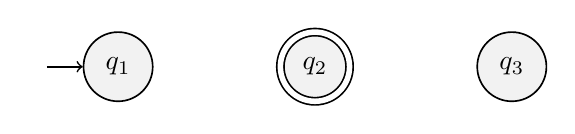
\begin{tikzpicture}
\node[state, initial] (q1) {$q_1$};
\node[state, accepting, right of=q1] (q2) {$q_2$};
\node[state, right of=q2] (q3) {$q_3$};
\end{tikzpicture}


{
.\newline\newline
}



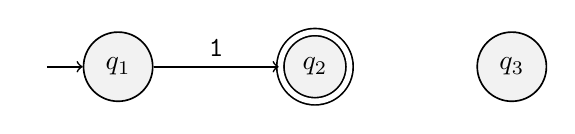
\begin{tikzpicture}
\node[state, initial] (q1) {$q_1$};
\node[state, accepting, right of=q1] (q2) {$q_2$};
\node[state, right of=q2] (q3) {$q_3$};
\draw (q1) edge node {\tt 1} (q2);
\end{tikzpicture}


{
.\newline\newline
}


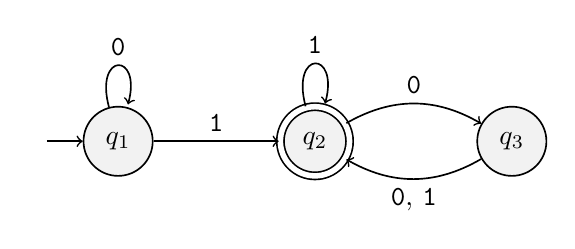
\begin{tikzpicture}
\node[state, initial] (q1) {$q_1$};
\node[state, accepting, right of=q1] (q2) {$q_2$};
\node[state, right of=q2] (q3) {$q_3$};
\draw (q1) edge[loop above] node {\tt 0} (q1);
\draw (q1) edge node {\tt 1} (q2);
\draw (q2) edge[loop above] node {\tt 1} (q2);
\draw (q2) edge[bend left] node {\tt 0} (q3);
\draw (q3) edge[bend left] node {{\tt 0}, {\tt 1}} (q2);
\end{tikzpicture}




{
.\newline\newline
}





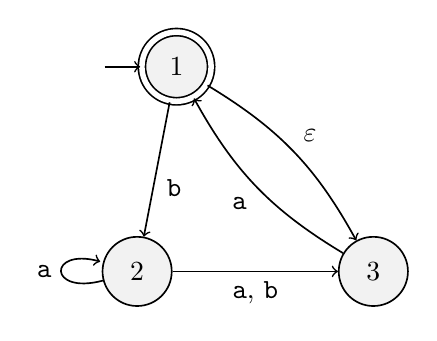
\begin{tikzpicture}
\node[state, initial, accepting] (1) at (.5,2.6) {$1$};
\node[state] (2) at (0,0) {$2$};
\node[state] (3) at (3,0) {$3$};
\draw (1) edge node{\tt b} (2);
\draw (1) edge[bend left=15] node {$\epsilon$} (3);
\draw (2) edge[loop left] node{\tt a} (2);
\draw (2) edge[below] node{{\tt a}, {\tt b}} (3);
\draw (3) edge[bend left=15] node{\tt a} (1);
\end{tikzpicture}



{
.\newline\newline\newline
}



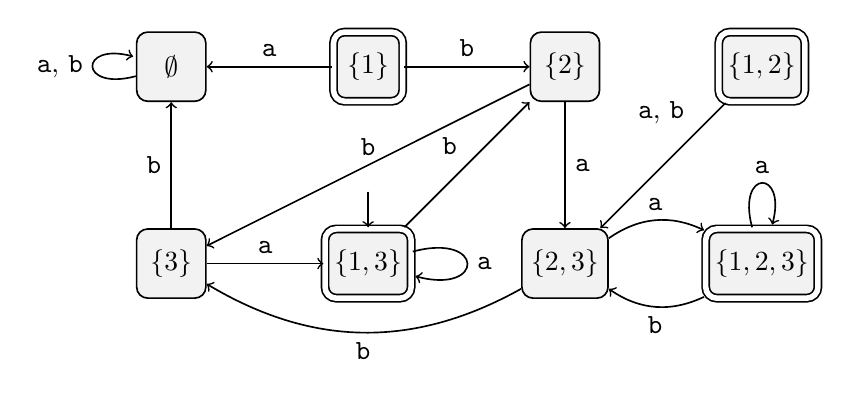
\begin{tikzpicture}
\tikzset{every state/.append style={rectangle, rounded corners}}
\node[state] (emp) {$\emptyset$};
\node[state, accepting, right of=emp] (1) {$\{1\}$};
\node[state, right of=1] (2) {$\{2\}$};
\node[state, accepting, right of=2] (12) {$\{1, 2\}$};
\node[state, below of=emp] (3) {$\{3\}$};
\node[state, initial, initial where=above, accepting, right of=3] (13) {$\{1, 3\}$};
\node[state, right of=13] (23) {$\{2, 3\}$};
\node[state, accepting, right of=23] (123) {$\{1, 2, 3\}$};
\draw (emp) edge[loop left] node {{\tt a}, {\tt b}} (emp);
\draw (1) edge[above] node {\tt a} (emp);
\draw (1) edge node {\tt b} (2);
\draw (2) edge node {\tt a} (23);
\draw (2) edge[above] node {\tt b} (3);
\draw (12) edge[auto=right,near start] node {{\tt a}, {\tt b}} (23);
\draw (3) edge node {\tt b} (emp);
\draw (3) edge node {\tt a} (13);
\draw (13) edge[loop right] node {\tt a} (13);
\draw (13) edge node {\tt b} (2);
\draw (23) edge[bend left,above] node {\tt a} (123);
\draw (23) edge[bend left] node {\tt b} (3);
\draw (123) edge[loop above] node {\tt a} (123);
\draw (123) edge[bend left,below] node {\tt b} (23);
\end{tikzpicture}



{
.\newline\newline\newline
}


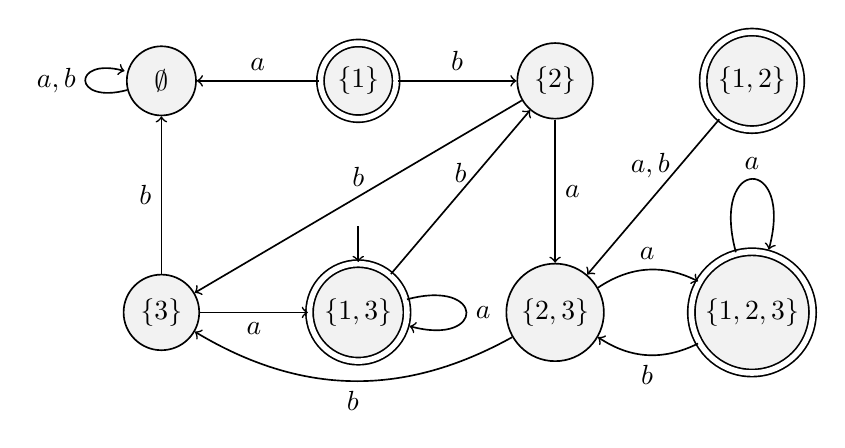
\begin{tikzpicture}
\node[state] (phi) {$\emptyset$};
\node[state, accepting, right of=phi] (1) {$\{1\}$};
\node[state, right of=1] (2) {$\{2\}$};
\node[state, accepting, right of=2] (12) {$\{1, 2\}$};
\node[state, below=2cm of phi] (3) {$\{3\}$};
\node[state, initial, initial where=above, accepting, right of=3] (13) {$\{1, 3\}$};
\node[state, right of=13] (23) {$\{2, 3\}$};
\node[state, accepting, right of=23] (123) {$\{1, 2, 3\}$};
\draw (phi) edge[loop left] node{$a, b$} (phi);
\draw (1) edge[above] node{$a$} (phi);
\draw (1) edge[above] node{$b$} (2);
\draw (2) edge[right] node{$a$} (23);
\draw (2) edge[above] node{$b$} (3);
\draw (12) edge[above, pos=.3, left=2pt] node{$a, b$} (23);
\draw (3) edge[left] node{$b$} (phi);
\draw (3) edge[below] node{$a$} (13);
\draw (13) edge[loop right] node{$a$} (13);
\draw (13) edge[above] node{$b$} (2);
\draw (23) edge[bend left, above] node{$a$} (123);
\draw (23) edge[bend left, below] node{$b$} (3);
\draw (123) edge[loop above] node{$a$} (123);
\draw (123) edge[bend left, below] node{$b$} (23);
\end{tikzpicture}





{
.\newline\newline\newline
}




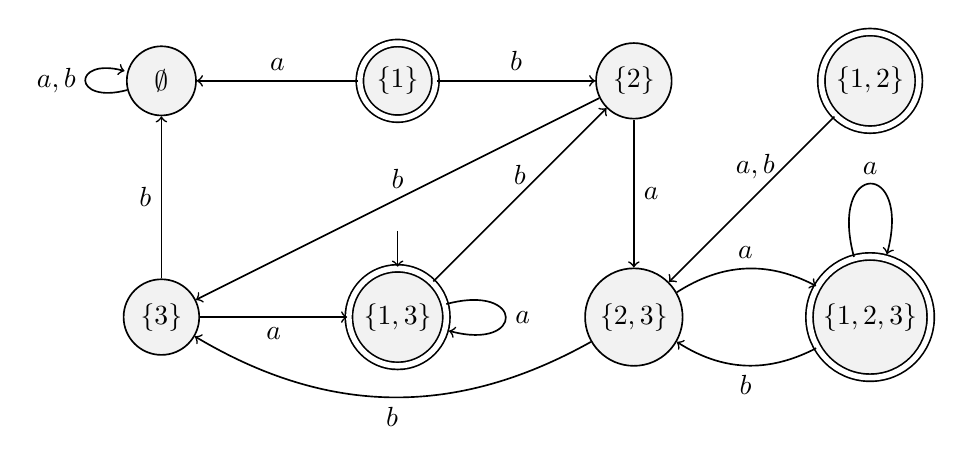
\begin{tikzpicture}
\tikzset{every state/.append style={node distance=3cm,shape=circle, rounded corners}}
\node[state] (phi) {$\emptyset$};
\node[state, accepting, right of=phi] (1) {$\{1\}$};
\node[state, right of=1] (2) {$\{2\}$};
\node[state, accepting, right of=2] (12) {$\{1, 2\}$};
\node[state, below of=phi] (3) {$\{3\}$};
\node[state, initial, initial where=above, accepting, right of=3] (13) {$\{1, 3\}$};
\node[state, right of=13] (23) {$\{2, 3\}$};
\node[state, accepting, right of=23] (123) {$\{1, 2, 3\}$};
\draw (phi) edge[loop left] node{$a, b$} (phi);
\draw (1) edge[above] node{$a$} (phi);
\draw (1) edge[above] node{$b$} (2);
\draw (2) edge[right] node{$a$} (23);
\draw (2) edge[above] node{$b$} (3);
\draw (12) edge[above, pos=.3, left=2pt] node{$a, b$} (23);
\draw (3) edge[left] node{$b$} (phi);
\draw (3) edge[below] node{$a$} (13);
\draw (13) edge[loop right] node{$a$} (13);
\draw (13) edge[above] node{$b$} (2);
\draw (23) edge[bend left, above] node{$a$} (123);
\draw (23) edge[bend left, below] node{$b$} (3);
\draw (123) edge[loop above] node{$a$} (123);
\draw (123) edge[bend left, below] node{$b$} (23);
\end{tikzpicture}







\end{document}